% -----------------------------------------------
% Template for ICMC 2005
%     icmc.sty -> style file
% By Eloi Batlle (eloi@iua.upf.es), changes for 
% ICMC by Bram de Jong (bdejong@iua.upf.es)
% -----------------------------------------------

\documentclass{article}
\usepackage{icmc,amsmath}
\usepackage{graphicx}

% Title.
% ------
\title{SndTools: Real-time Audio DSP and 3D Visualization}

% Single address
% To use with only one author or several with the same address
% ---------------
\oneauthor
{Ananya Misra \quad Ge Wang \quad Perry R. Cook$^{\dag}$} {Princeton University \\ Department of Computer Science ($^{\dag}$also Music)}

% Two addresses
% --------------
%\twoauthors
%  {First author} {School \\ Department}
%  {Second author} {Company \\ Address}

% Three addresses
% --------------
%\threeauthors
% {First author} {School \\ Department}
%  {Second author} {Company \\ Address}
%  {Third author} {Company \\ Address}

\begin{document}
%
\maketitle
%

\begin{figure}[t!]
\center
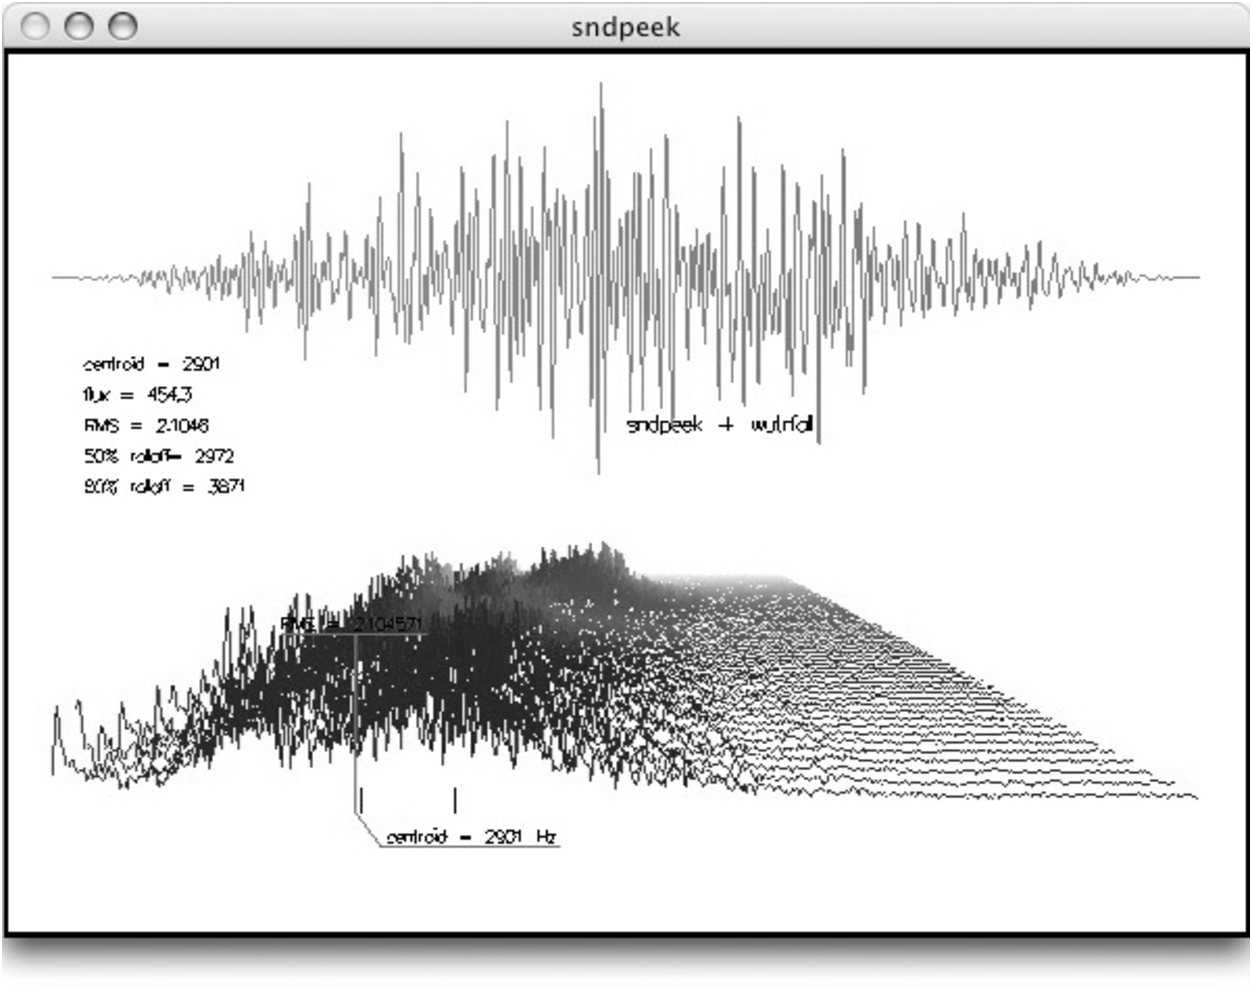
\includegraphics[width=\columnwidth]{sndpeek3_bw}
%\caption{Views of {\bf sndpeek}}
%\label{fig:f_teaser}
\end{figure}

\begin{abstract}
We present {\bf sndtools}, a set of cross platform, open-source tools for simultaneously displaying related audio and visual information in real-time. The distribution includes tools to extract spectral information, perform linear predictive coding analysis and resynthesis, manipulate pitch and time using a phase vocoder, and map text to Morse code. Each tool has closely related audio and visual (graphical or text) components and can be used for instructive purposes or experimentation with sound. We show that hardware-accelerated graphics tools such as OpenGL can be used to enable real-time 3D visualization of DSP algorithms. 
%The components that combine graphical displays with substantial computation make use of %hardware-accelerated graphics tools. 
\end{abstract}
%
\section{Motivation}

Advances in computer graphics rendering have made it possible to render large amounts of information at high 
speed and low cost. The graphics environment OpenGL, for example, offers powerful hardware-accelerated computation, 
with common functions, such as rotation, scaling and lighting, optimized to take up few resources. In addition, its 
widespread support across platforms allows OpenGL programmers to take advantage of standard library routines.
%, and still compile and run on many different platforms. (uh, this is what support across
% platforms means)
The programming interface also provides flexibility to 
design customized widgets and displays. This suggests that both the power and the flexibility of OpenGL can be 
leveraged to create cross-platform real-time sound visualization displays.

\begin{figure}
\center
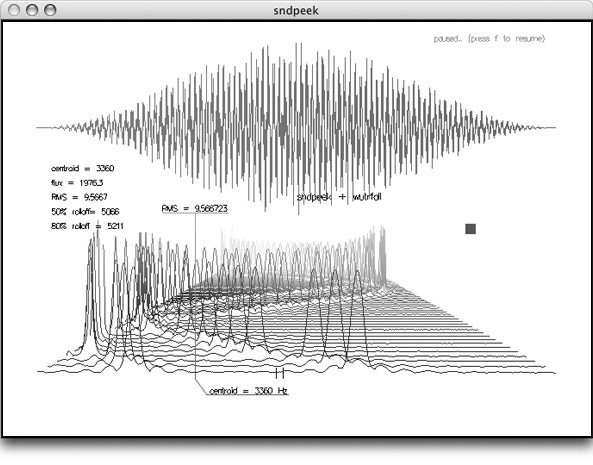
\includegraphics[width=\columnwidth]{sndpeek2_bw}
%\caption{{\bf sndpeek} in action.}
%\label{fig:f_sndpeek}
\end{figure}

Existing audio visualization tools are often not real-time. Those that are \cite{Lauer:03, Deadlinks:05}, 
tend not to use hardware-accelerated graphics tools, which limits the complexity of audio and visual computations they can perform. They are also often designed for a specific platform and are difficult to port.

The {\bf sndtools} package presents several real-time audiovisual displays that take advantage of efficient graphics tools 
to devote more processing power to audio analysis and synthesis. Thus, complex operations such as spectral feature 
extraction, linear predictive coding and phase vocoder-based pitch and time manipulations can be performed and 
visualized in real-time. As a side effect of this processing freedom, the package also provides a reusable library 
of analysis and synthesis tools. 
\sloppy
All the programs in the {\bf sndtools} distribution are open source and run on most popular platforms, including MacOS X, 
Windows and Linux. (Visit URL provided at end of paper for source code and executables.) Thus, {\bf sndtools} subscribes to 
%[lives up to, is an example of, supports, embraces, upholds, follows, ?] 
the notion of free sound, where "free" can mean both "no-cost" 
and, more generally, "accessible". We hope this accessibility encourages users to experiment with the tools provided. 

\begin{figure*}
\center
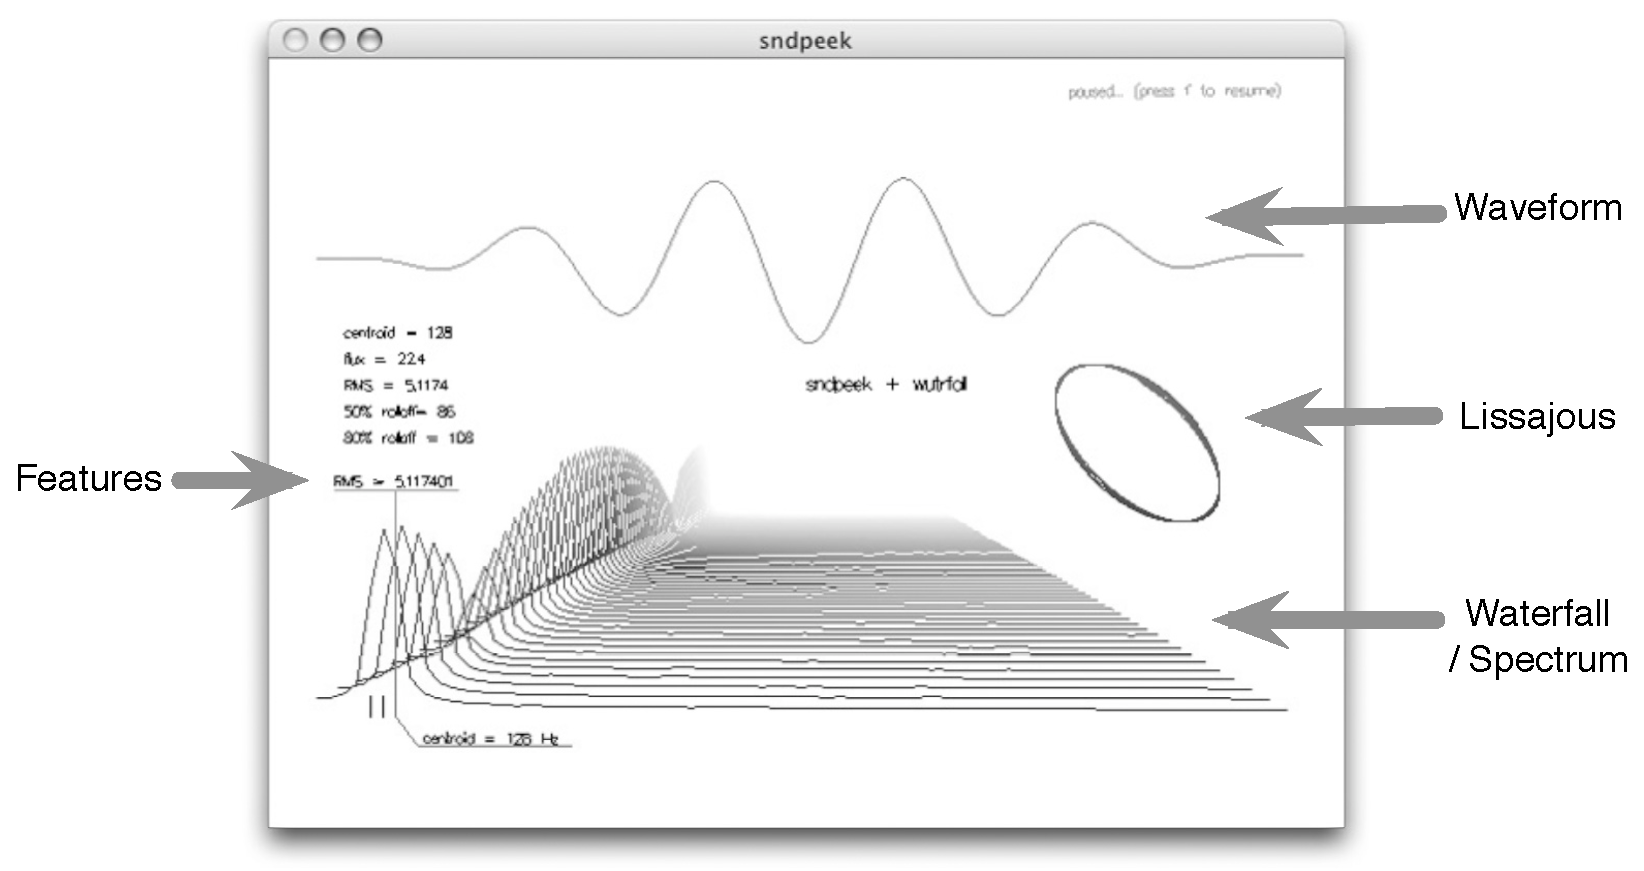
\includegraphics[width=\textwidth]{sndpeek_bw}
\caption{{\bf sndpeek} in action.}
\label{fig:f_sndpeek}
\end{figure*}

In the rest of this paper, we describe the components of the {\bf sndtools} distribution. {\bf sndpeek} is a waveform and 
spectrum visualizer with several other features. {\bf rt\_lpc} performs linear predictive coding to analyze and 
synthesize sound and displays the results visually as well as via audio output. {\bf rt\_pvc} is a phase vocoder that also has 
real-time display.
{\bf morse} translates text to Morse code and provides a text visualization of the result, synchronized with audio. Although it does not rely on high-level graphics tools, it resembles the other components in computing and simultaneously presenting related visual and audio information. 
% {\bf Morse} [does not use OpenGL] provides an ASCII visualization and audio rendering of Morse code and 
%thus seems unrelated to the rest of this, but it is too cool to omit. 
We then conclude and describe possibilities for future work.

%two parts: 
%visualizing sound in different ways, and 
%library of analysis/synthesis tools;

%free sound!  the programs in the sndtools distribution are all open source, and cross platform
%(MacOS X, Windows, Linux)

%opengl is good
%  - cross platform
%  - out of the box (standard in every platform) / easy compilation / library handling
%  - powerful - free rotation and scaling and lighting
%  - flexible - free to design custom widgets and displays
%  - hardware accelerated

\section{sndpeek}

{\bf sndpeek} performs spectral analysis on audio input and displays the information graphically. Figure 1 shows a screen shot of {\bf sndpeek} in action. 

%[figure] with things pointing at features

In essence, {\bf sndpeek} provides real-time 3D visualization of components including:
\begin{itemize}
\setlength{\itemsep}{-2pt}
\item \textit{Time-domain waveform}, which can be input from a microphone 
or from a .wav, .aiff, .snd, .raw, or .mat file with optional playback. 
\item \textit{FFT magnitude spectrum} scaled by a weighted square root function so that peaks are easier to decipher than with linear or dB scaling
\item \textit{3D waterfall plot} - cascading FFT magnitude spectra where previous frames fade into the background
\item \textit{Lissajous plot} showing correlation between the left and right channels (stereo signals), or {\it phase delay similarity plot} showing the signal versus a delayed version of itself (for mono signals)
\item \textit{Spectral features} - features such as centroid, rms, rolloff and flux are extracted using the MARSYAS framework \cite{Tzanetakis:00} and displayed in real-time
\end{itemize}

The display itself can be manipulated in several ways. Options include scaling and rotating the display to facilitate zooming in on information from different viewpoints, and the ability to freeze the display on a single frame for closer observation. The spacing between spectra in the waterfall plot can also be modified, and the spectrum view can be toggled between dB and the default scaling. 

%\item \textit{Rotatable and scalable display} to facilitate observation from different viewpoints
%\item \textit{Freeze frame} - freezes the display on a single frame for more detailed observation
%\end{itemize}

%Sndpeek runs on MacOS X, Linux, and Windows under GPL and can be freely downloaded from [somewhere]. The 
%source is also freely available. free sound

{\bf sndpeek} can also be adapted for use in other systems. For example, it is an 
%indispensable, essential, salient 
essential part of the Audicle \cite{Wang:04}. 

\section{rt\_lpc}

\begin{figure*}[t]
\center
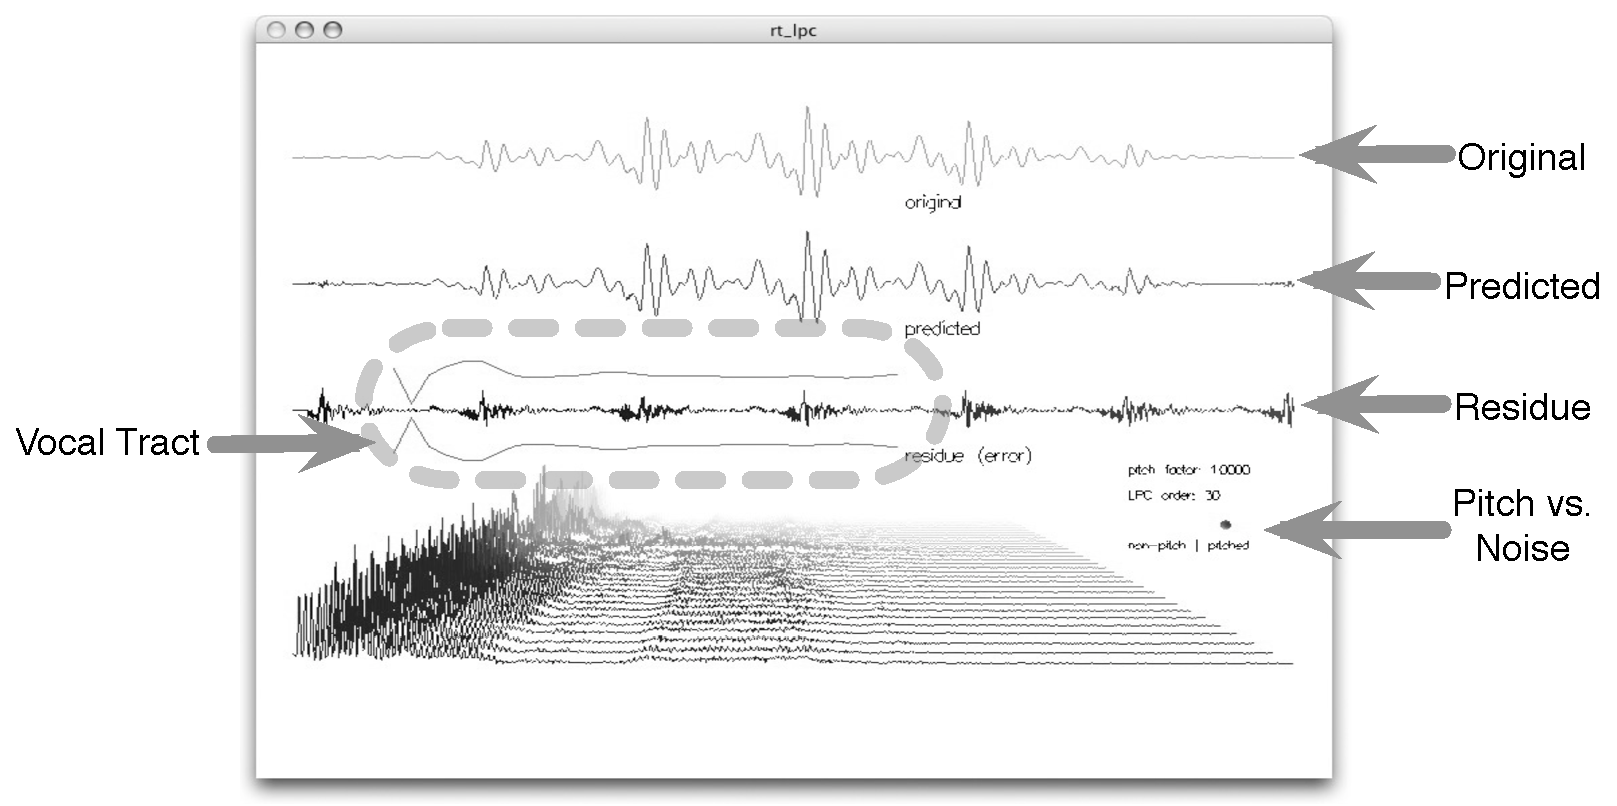
\includegraphics[width=1\textwidth]{rt_lpc_bw}
\caption{{\bf rt\_lpc}: real-time LPC analysis and resynthesis.}
\label{fig:f_lpc}
\end{figure*}

{\bf rt\_lpc} performs real-time linear predictive coding (LPC) \cite{Atal:70, Lansky:81, Markel:76, Moorer:79} analysis and resynthesis on audio input. The input sound is analyzed to obtain a number of filter coefficients and an error signal, as well as a pitch estimation. The coefficients are then used to synthesize and play back in real-time a signal close to the original sound. The controls available can be used for pedagogical purposes to show how different variables affect the LPC analysis and synthesis, or for fast trial-and-error to obtain the optimal settings for some desired output. 

%[figure]

The visual components of the display include: 
\begin{itemize}
\setlength{\itemsep}{-2pt}
\item \textit{Original waveform} - the waveform of the input sound
\item \textit{Predicted waveform} - the waveform predicted by the LPC coefficients
\item \textit{Error waveform} - difference between the original and the predicted waveforms
\item \textit{Vocal tract shape visualization} obtained from the LPC coefficients using Durbin Recursion \cite{Durbin:60}. 
\item \textit{Pitch} - whether the sound is pitched or unpitched
\item \textit{FFT magnitude spectrum and waterfall plot} and other features from {\bf sndpeek}
\item \textit{Information} on the current values of adjustable parameters. These include:\\
	-- {\it LPC order} - the number of coefficients analyzed\\
	-- {\it Pitch shift factor} - for pitched sounds, the pitch can be modified by some factor before synthesis 
\end{itemize}

In addition, the pitch pulse source can be selected to provide an impulse or to model a glottal pulse. Optional emphasis and deemphasis filters can also be applied before and after the LPC is performed. 

Apart from real-time LPC visualization, {\bf rt\_lpc} also offers a modular LPC library for use in other applications. The library consists of an LPC data structure, \textit{analyze} and \textit{synthesize} functions, and several helper units. 

%[real-time LPC analysis
%real-time LPC synthesis
%visualization of original, predicted, and error waveforms
%visualization of vocal tract shape from LPC coefficients
%adjustable LPC analysis order
%adjustable synthesis pitch shift
%lots of other choices (pitch pulse source selection, emphasis filter)
%STFT plot
%modular LPC library
%available on MacOS X, Linux, and Windows under GPL
%
%more about library]
%
%[figure]

\section{rt\_pvc}

{\bf rt\_pvc} is a real-time phase vocoder \cite{Dolson:86, Moorer:78} that can be used to time-stretch and pitch-shift sound while minimizing artifacts arising from phase incoherence. It computes the FFT spectrum for each windowed frame of input audio, and carries out pitch-shifting and time-stretching by manipulating consecutive spectra. It then performs phase adjustment to account for discrepancies caused by moving the bins and frames in the previous step. 

Since the phase vocoder is real-time, time stretching and compression can cause changes in delay in the playback. The tool keeps track of this delay, allowing the synthesis to fall behind or catch up with the live input. 

\begin{figure}
\center
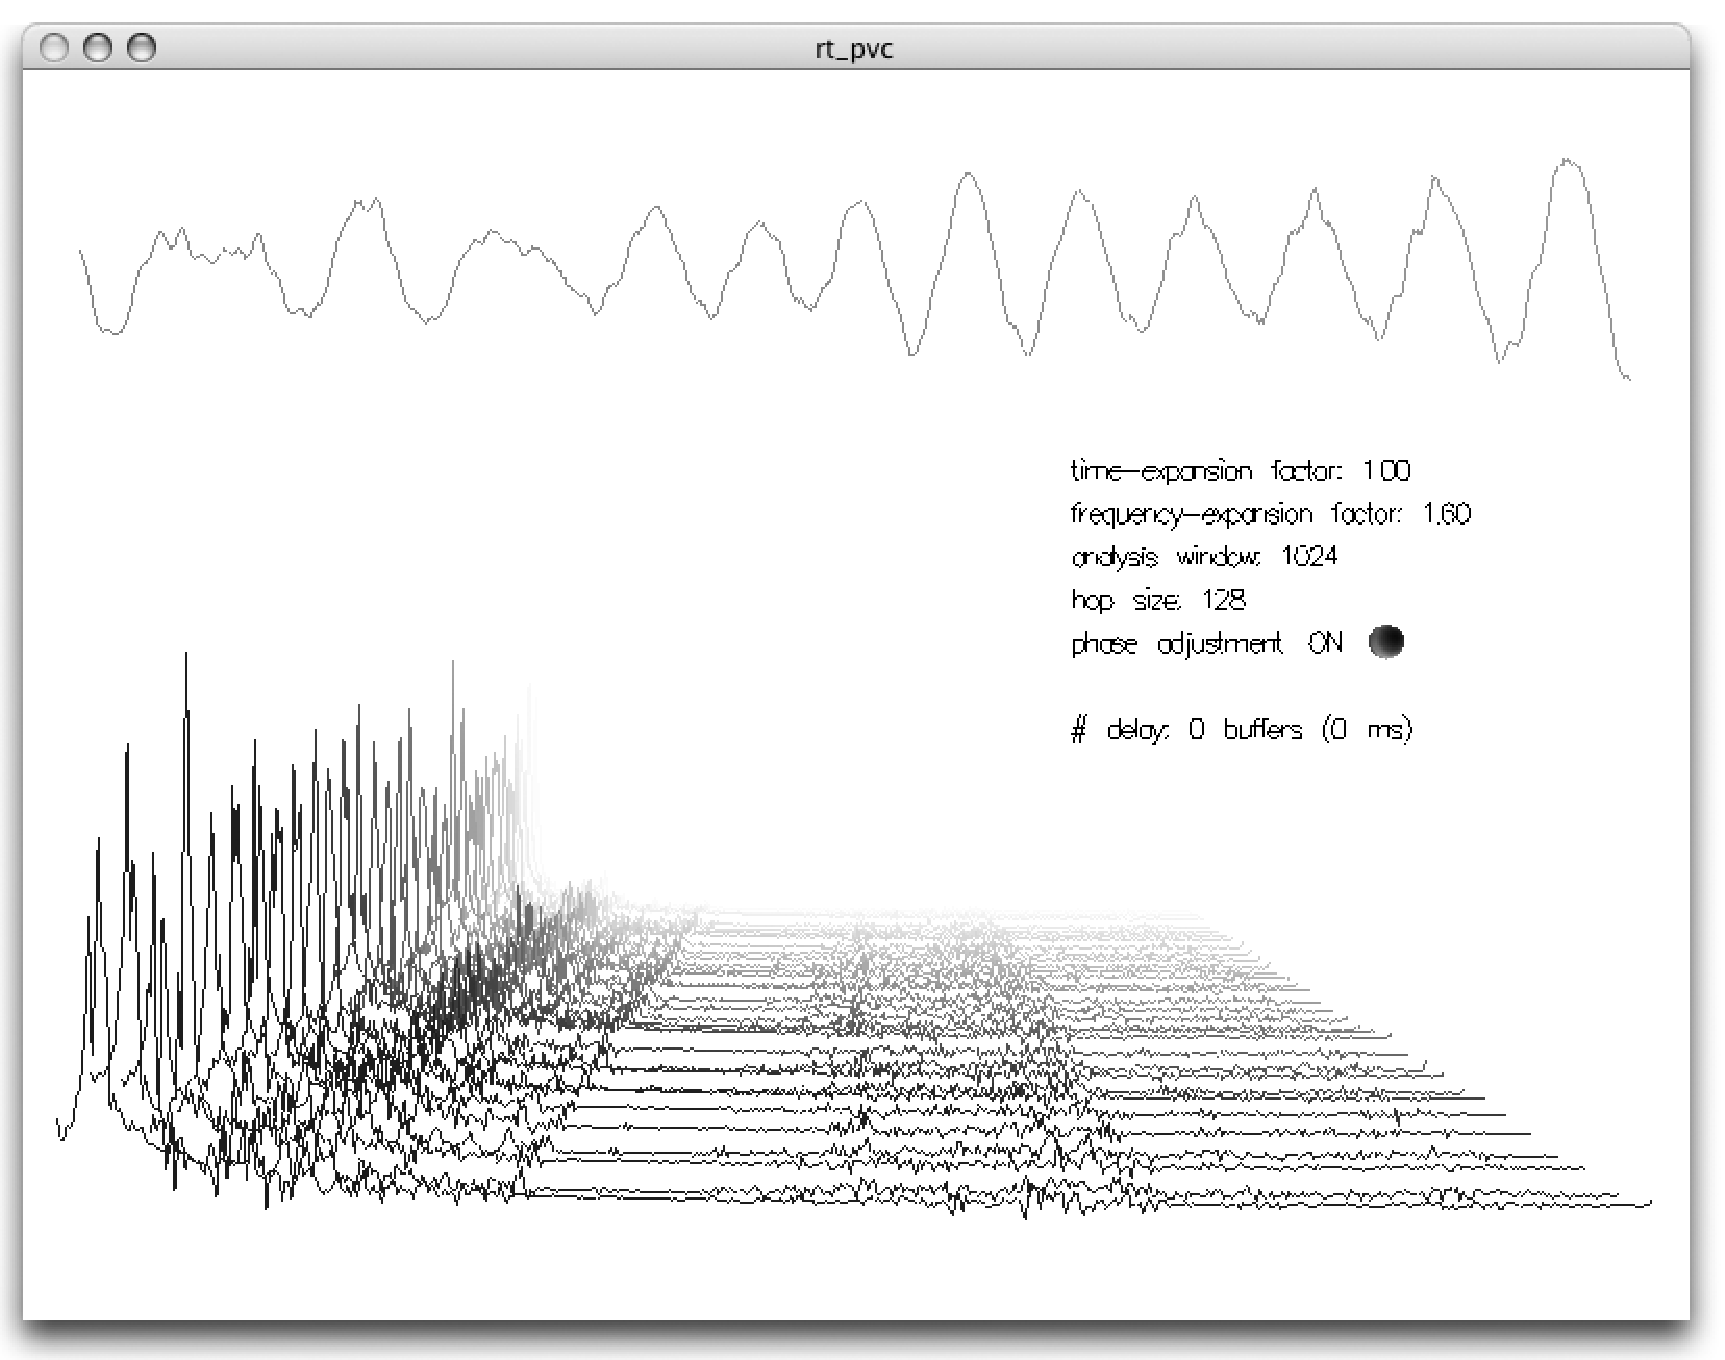
\includegraphics[width=\columnwidth]{rt_pvc_bw}
\caption{{\bf rt\_pvc}: real-time phase vocoder.}
\label{fig:f_pvc}
\end{figure}

The visual display includes: 
\begin{itemize}
\setlength{\itemsep}{-2pt}
\item \textit{Original waveform} - the waveform of the input sound
\item \textit{FFT magnitude spectrum and waterfall plot} similar to the {\bf sndpeek} display
\item \textit{Information} on the current parameter values, including:\\
	-- {\it Time-expansion factor} - adjustable amount by which the signal is lengthened (or shrunk) in time\\
	-- {\it Frequency-expansion factor} - adjustable factor for changing frequency or pitch\\
	-- {\it Analysis window size} - the length of sound analyzed as one frame\\
	-- {\it Hop size} - adjustable spacing between the beginnings of consecutive analysis windows\\
	-- {\it Phase adjustment} - the option to adjust phase or not, for demonstrating the difference made by phase adjustment\\
	-- {\it Buffer delay} - the delay accumulated so far due to time-stretching 
\end{itemize} 

Like {\bf rt\_lpc}, {\bf rt\_pvc} can be used for both pedagogical purposes and for testing the effects of changing parameters in real-time. Moreover, it also offers a modular phase vocoder library for use elsewhere. The library contains {\it analyze} and {\it synthesize} functions as well as functions for phase fixing and unwrapping, frequency shifting, overlap add (for time-stretching), and cross synthesis. It also includes helper functions for windowing and for handling multiple buffers. 

%real-time phase vocoder
%makes sense for pitch shifting
%time stretching - buffered approach

\section{morse}

{\bf morse}, a barely nontrivial but fun command-line utility, reads in text and outputs the Morse code version of it as ASCII dots and dashes. These are mapped to short and long beeps, which are played in real-time by synchronizing the printing of each symbol with the playing of the associated sound.

Here is an example of {\bf morse} at work. 
\begin{verbatim}
> morse
Type characters (case insensitive)
free sound
FREE SOUND
..-. .-. . .   ... --- ..- -. -.. 
\end{verbatim}

In this example, the user begins the {\bf morse} program and types in "free sound". The program reprints the input in Roman characters and in Morse code. The Morse code version is accompanied by the corresponding sounds. While the association with sound can make learning Morse code easier and more interesting, the program has also been used in computer music performances.

\section{conclusions}

Taking advantage of widely available computer graphics tools allows us to efficiently render visual displays, freeing more resources for audio analysis, manipulation and synthesis. This allows real-time visualization and audio processing to take place simultaneously, even for relatively complex analysis and synthesis operations. Built on this premise, {\bf sndtools} offers real-time audio and visual display of common sound manipulation tools such as spectral analysis, LPC and phase vocoders. It also provides libraries of these tools, as well as other %(supplementary?) 
mini-tools that can be used for instruction, composition or just for fun. 

Plans for future work involve integrating more tools into the distribution. New tools can include both real-time 3D visualizations of other common audio analysis and synthesis algorithms, as well as interesting smaller-scale units. Our final goal is to have a comprehensive set of open-source, cross-platform, real-time sound tools.\\\\\\\\\\\

%our results support our hypothesis.  what is our hypothesis?
%every paper should have one. or at least a thesis. 

%opengl is good
%  - cross platform
%  - out of the box / easy compilation / library handling
%  - powerful - free rotation and scaling and lighting
%  - flexible - free to design custom widgets and displays
%  - hardware accelerated
\section{acknowledgements}

We thank Ahmed Abdallah and Paul Botelho for co-authoring {\bf rt\_pvc}, and Matthew Hoffman for code and ideas on {\bf rt\_lpc}.  
%We also thank Frances Spalding, Iannis Tourlakis, and Limin Jia, for feeding us.
\smallskip

\center{SndTools is open-source and freely available at:}
\center{
\texttt{http://sndtools.cs.princeton.edu/}
}
\smallskip

\begin{thebibliography}{11}


%\bibitem{Author:00} Author, E.
%''The title of the conference paper'',
%{\it Proceedings of the International Computer Music Conference}, Miami, USA, 2004.
%
%\bibitem{Someone:02} Someone, A.
%{\it  Title of the book}.
%Editorial Acme, Barcelona, 2005.
%
\bibitem{Atal:70} Atal, B.
"Speech Analysis and Synthesis by Linear Prediction of the Speech Wave",
{\it Journal of the Acoustical Society of America 47.65(Abstract)}, 1970.

\bibitem{Dolson:86} Dolson, M. 
"The Phase Vocoder: A Tutorial",  
{\it Computer Music Journal 10(4):14-27}, 1986.

\bibitem{Durbin:60} Durbin, J.
"The Fitting of Time-Series Models", 
{\it Rev. Inst. Int. Stat. 28(3):233-243}, 1960.

\bibitem{Lansky:81} Lansky, P. and K. Steiglitz.  
"Synthesis of Timbral Families by Warped Linear Prediction",
{\it Computer Music Journal 5(3):45-49}, 1981.

\bibitem{Lauer:03} Lauer, C. and N. Reithinger. 
"A Lightweight Configurable Signal Analysis Toolset for Multiple Applications",
{\it Proceedings of the International Conference on Acoustics, Speech, and Signal Processing (ICASSP)}, 2003.

\bibitem{Markel:76} Markel, J. and A. Gray. 
{\it Linear Prediction of Speech}.
Springer, New York, 1976.

\bibitem{Moorer:79} Moorer, J. 
"The Use of Linear Prediction of Speech in Computer Music Applications",
{\it Journal of the Audio Engineering Society 27(3):134-140}, 1979.

\bibitem{Moorer:78} Moorer, J.
"The Use of the Phase Vocoder in Computer Music Applications",
{\it Journal of the Audio Engineering Society 26(1/2):42-45}, 1978.

%\bibitem{Rabiner:78} Rabiner, L. R. and Schafer, R. W.
%{\it Digital Processing of Speech Signals}.
%Prentice-Hall (Signal Processing Series), 1978.

\bibitem{Deadlinks:05} 
"Scopes and Realtime Visualizers", 
From http://www.linux-sound.org/scopes.html, 
Retrieved March 5, 2005.

\bibitem{Tzanetakis:00} Tzanetakis, G., and P. R. Cook.
"MARSYAS: A Framework for Audio Analysis",
{\it Organised Sound 4(3)}, 
Cambridge University Press, 2000. 

\bibitem{Wang:04} Wang, G. and P. R. Cook.
"The Audicle: a Context-sensitive, On-the-fly Audio Programming
Environ/mentality",
{\it Proceedings of the International Computer Music Conference  (ICMC)},
Miami, USA, 2004.

\end{thebibliography}

\end{document}
